% IEEEAerospace2012.cls requires the following packages: times, rawfonts, oldfont, geometry
\documentclass[twocolumn,letterpaper]{IEEEAerospaceCLS}  % only supports two-column, letterpaper format
%\setcounter{tocdepth}{3}

% The next line gives some packages you may find useful for your paper--these are not required though.
%\usepackage[]{graphicx,float,latexsym,amssymb,amsfonts,amsmath,amstext,times,psfig}
% NOTE: The .cls file is now compatible with amsmath!!!

\usepackage[]{graphicx}    % We use this package in this document
\newcommand{\ignore}[1]{}  % {} empty inside = %% comment

% The following packages can be found on http:\\www.ctan.org
%\usepackage{graphics} % for pdf, bitmapped graphics files
%\usepackage{epsfig} % for postscript graphics files
%\usepackage{mathptmx} % assumes new font selection scheme installed
%\usepackage{times} % assumes new font selection scheme installed
\usepackage{amsmath} % assumes amsmath package installed
\usepackage{amssymb}  % assumes amsmath package installed

\usepackage{comment}
\usepackage{xcolor}
\usepackage{todo}
\usepackage{tabularx}

\usepackage{hyperref}

\usepackage{lipsum}
\usepackage{stfloats}
\usepackage{siunitx}

\usepackage{svg}

%\usepackage{hhline}

\usepackage[style=ieee]{biblatex}
\addbibresource{references.bib}
\addbibresource{jbowkett.bib}

%comment out below and uncomment block below below to remove all author location tags
\newcommand{\marco}[1]{{\color[HTML]{87E0CF}\textbf{Marco ToDo: #1}}}
\newcommand{\joseph}[1]{{\color{green}\textbf{Joseph ToDo: #1}}}
%\newcommand{\marco}[1]{}
%\newcommand{\joseph}[1]{}

\begin{document}
\title{A High-Fidelity Actuator Model for Robotic Autonomy in Space and Beyond}

\author{Preston Rogers, Joseph Bowkett, Paul Backes \\
\\
NASA Jet Propulsion Laboratory\\
California Institute of Technology\\
Pasadena, CA 91011\\
preston.rogers@jpl.nasa.gov%
%\thanks{The authors are with the NASA Jet Propulsion Laboratory, California Institute of Technology, 4800 Oak Grove Dr, Pasadena, CA 91109, USA.~Contact: {\tt\small bowkett@jpl.nasa.gov}}%
%\thanks{The  research  described  in  this  paper  was  carried  out  at  the  Jet  Propulsion  Laboratory,  California  Institute  of  Technology,  under  a  contract  with the  National  Aeronautics  and  Space  Administration. \copyright~2020 California Institute of Technology. Government sponsorship acknowledged.}%
%%%% IMPORTANT: Use the correct copyright information--IEEE, Crown, or U.S. government. %%%%%
\thanks{\footnotesize 979-8-3315-7360-7/26/$\$31.00$ \copyright2026 IEEE}
              % This creates the copyright info that is the correct 2026 data.
%\thanks{{U.S. Government work not protected by U.S. copyright}}         % Use this copyright notice only if you are employed by the U.S. Government.
%\thanks{{979-8-3503-0462-6/24/$\$31.00$ \copyright2024 Crown}}          % Use this copyright notice only if you are employed by a crown government (e.g., Canada, UK, Australia).
%\thanks{{979-8-3503-0462-6/24/$\$31.00$ \copyright2024 European Union}}    % Use this copyright notice is you are employed by the European Union.
}

\begin{comment}
    KEY NOTE: The overarching goal of this paper is to distill the status of the In-Contact Manipulation formulation and modeling for reference purposes. Also, secondarily, to get it published.

    Another note: each sentence is placed on a different line to make it easier to see differences in content between versions, as the back-end of overleaf version control is git. Blocking sentences into entire paragraphs means a one word change turns into a block of text change.
\end{comment}

\maketitle

\thispagestyle{plain}
\pagestyle{plain}

\begin{abstract}
This work presents a generalized actuator modeling approach that enhances simulation accuracy, with applications extending beyond Mars exploration. Actuators are integral components in space robotics, where precision and reliability are paramount. The circa-2023 Sample Retrieval Lander (SRL) design exemplifies this, relying on a robotic arm to retrieve Mars sample tubes for return to Earth. With Earth–Mars round-trip communication delays on the order of minutes, direct human teleoperation is unsafe and impractical, necessitating autonomous execution through onboard kinematic controllers. Because the robotic arm represents a single point of failure in such a critical mission, we develop an exceptionally high-fidelity simulation environment to validate the controller design. Unlike many system simulations that idealize actuator performance to simplify computations, our model captures key dynamics often overlooked in traditional approaches. Its accuracy is validated through comparisons with real-world actuator tests, demonstrating both mission relevance for SRL and potential applicability to future space robotics systems.
\end{abstract}

\section*{Nomenclature}

\begin{table}[h!]
\renewcommand{\arraystretch}{1.1}
\centering
\begin{tabular}{l l}
\hline
\textbf{Symbol} & \textbf{Description} \\
\hline
$ \theta_m $ & Motor angle before gear reduction \\
$ \theta_o $ & Output shaft angle \\
$ i_q $ & Active current \\
$ k_t $ & Torque constant \\
$ g_r $ & Gear ratio \\
$ \delta $ & Backlash gap angle \\
$ J_m, B_m $ & Motor inertia and damping \\
$ J_o, B_o $ & Output shaft inertia and damping \\
$ K_{\text{stiff}}, B_{\text{stiff}} $ & Stiffness and damping coefficients \\
$ \tau_{\text{mech}} $ & Mechanical torque \\
$ \tau_{\text{cogging}} $ & Cogging torque \\
$ \Delta \theta $ & Torsional deflection of output shaft \\
$ \tau_{\text{in}} $ & Torque at the start of the output shaft \\
$ \tau_{\text{out}} $ & Torque at the end of the output shaft \\
$ \tau_f, \tau_s $ & Kinetic and static friction torque \\
$ \mu_f, \mu_s  $ & Kinetic and static friction coefficients \\
$ \alpha_s $ & Stribeck decay coefficient \\
$ \tau_{\text{friction}} $ & Stribeck friction torque \\
$ \tau_{\text{ext}} $ & External torque \\
$ \sigma, \sigma_{\text{resolver}} $ & Hall and resolver standard deviations \\
$ \theta^{(\text{sensed})} $ & Angle measurement from resolver \\
$ \dot{\theta}^{(\text{sensed})} $ & Velocity measurement from halls \\
\hline
\end{tabular}
\end{table}




\tableofcontents

%%%%%%%%%%%%%%%%%%%%%%%%%%%%%%%%%%%%%%
\section{Introduction} 
%%%%%%%%%%%%%%%%%%%%%%%%%%%%%%%%%%%%%%
From the Hubble Space Telescope capturing the birth of stars to Viking 1 conducting the first regolith analysis on Mars, autonomous systems have played a pivotal role in expanding our understanding of the universe. These autonomous explorers test scientific theories, deepen our knowledge of Earth, and pave the way for future human exploration beyond our planet.


\begin{figure}[!b]
\centering
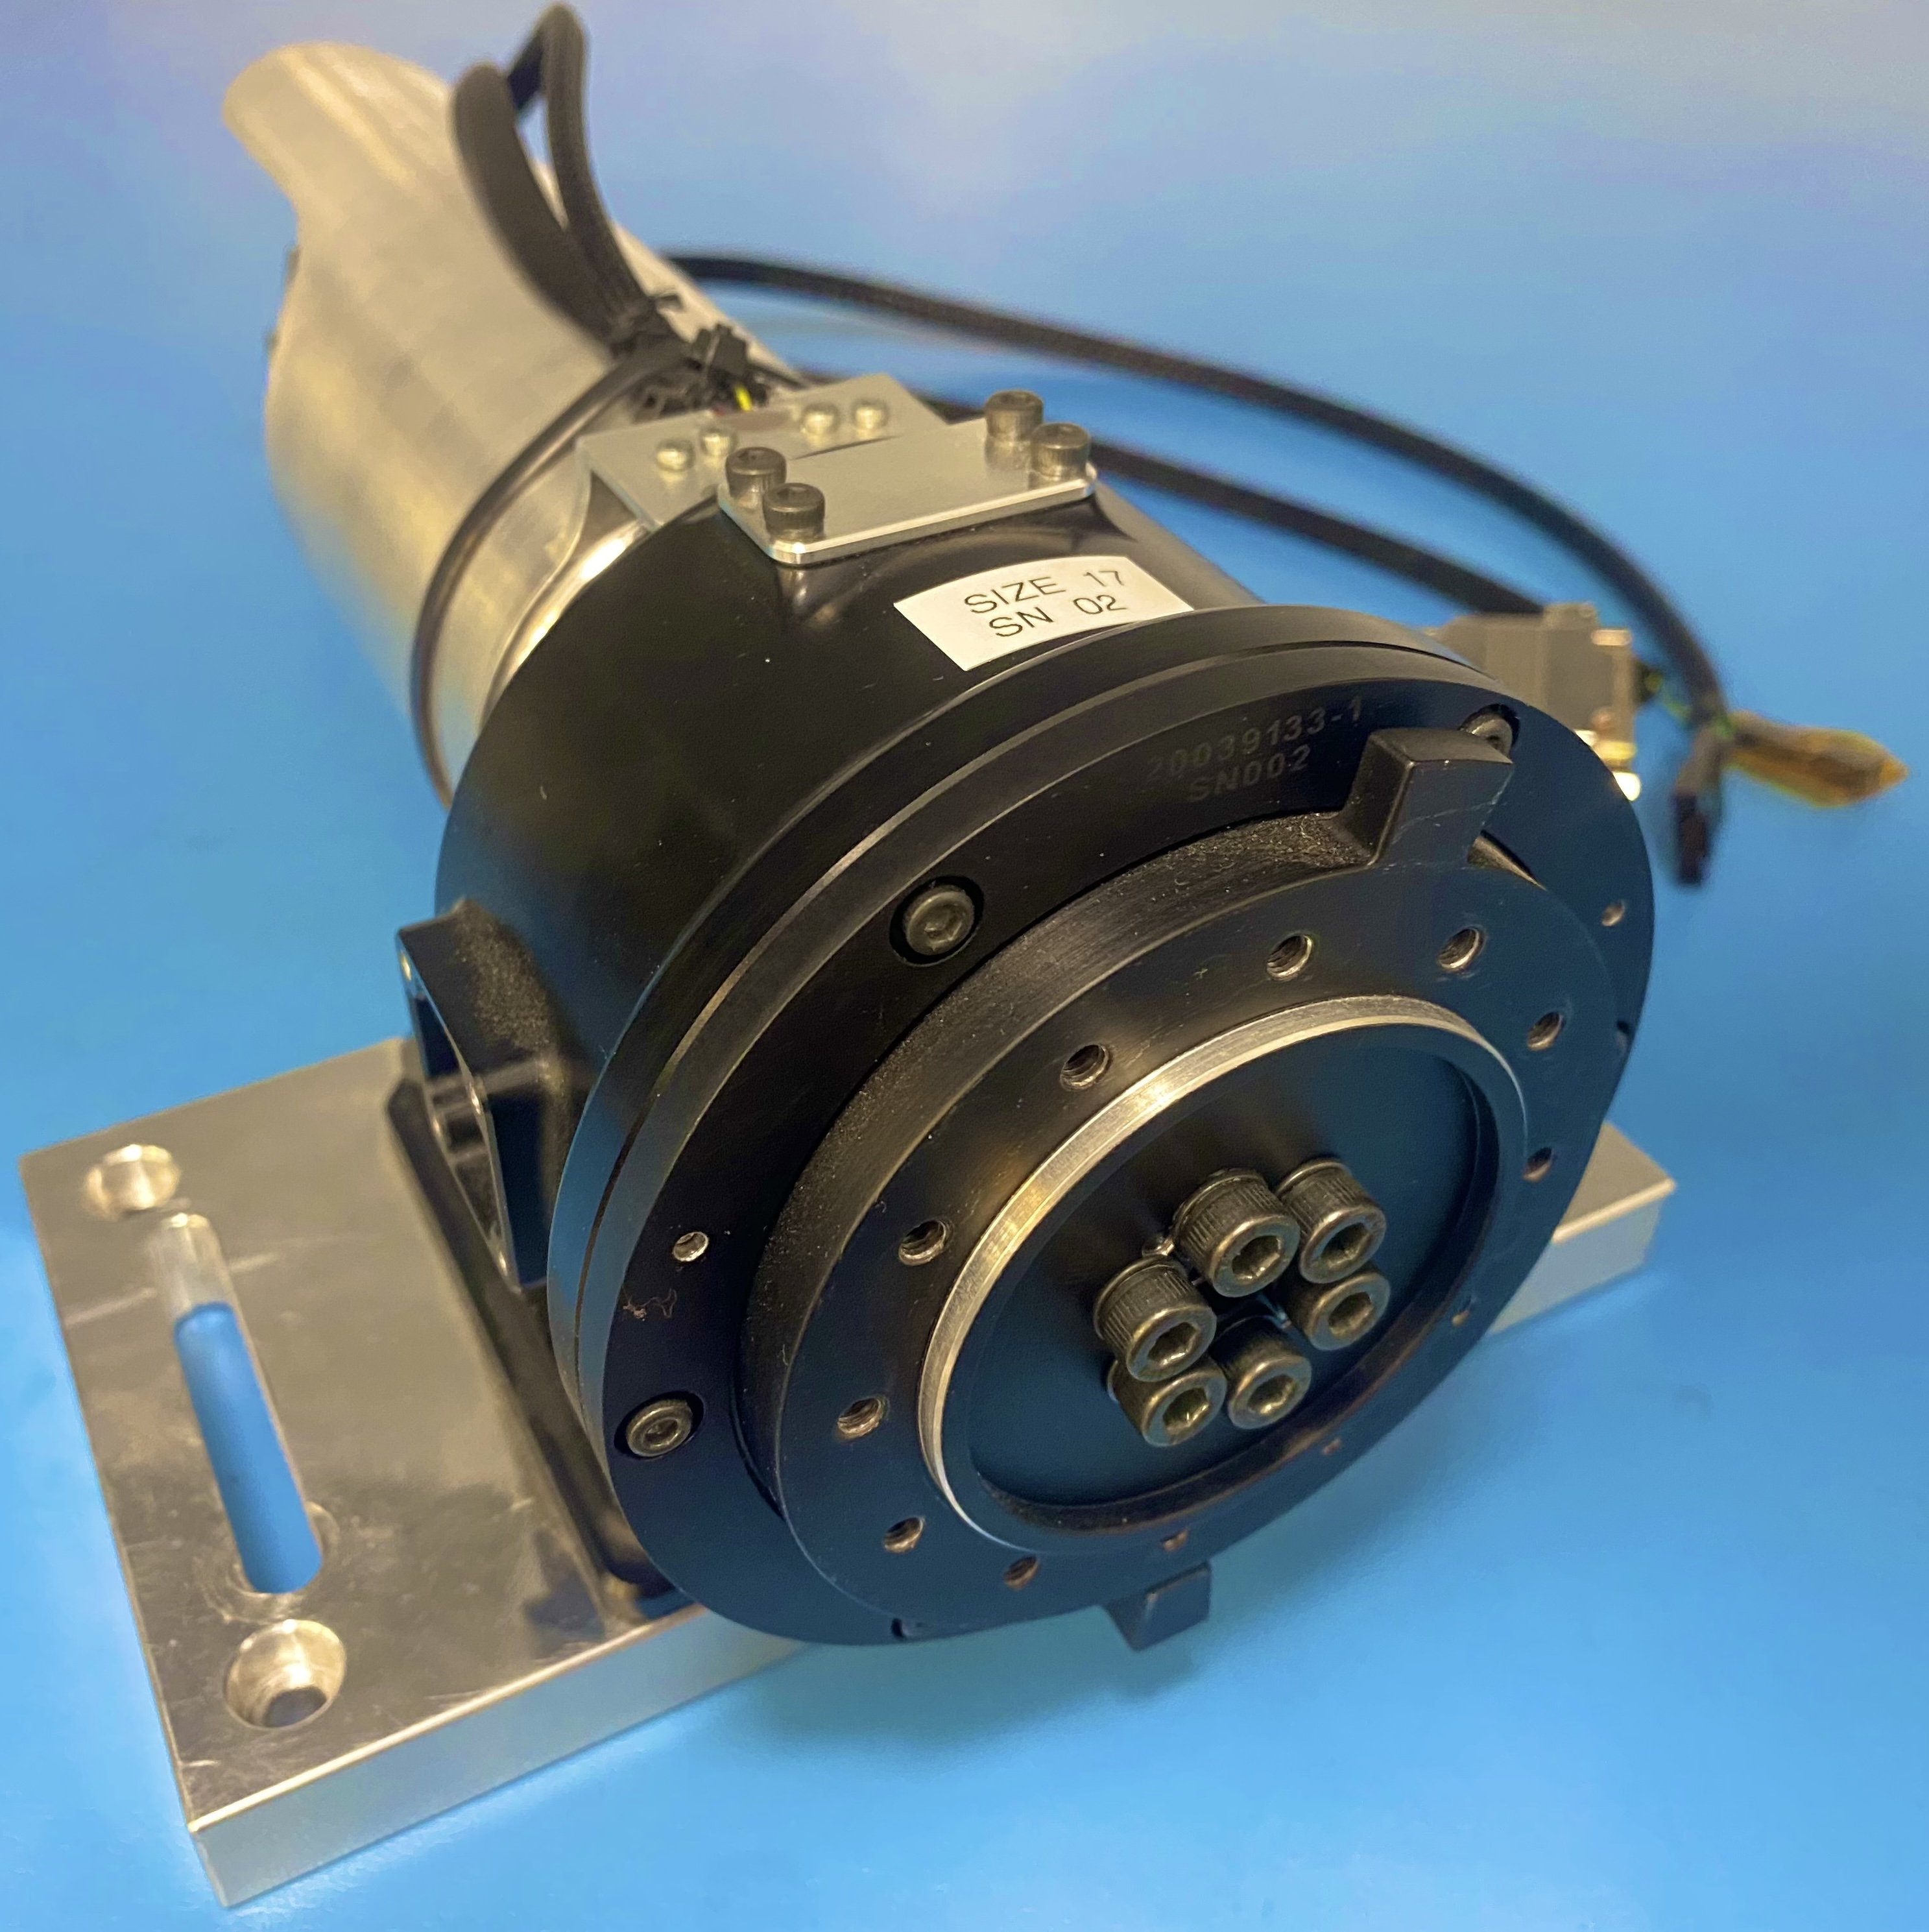
\includegraphics[width=0.9\columnwidth]{images/actuator_picture.jpg}
\caption{Picture of an actuator from the `Bradbury' testbed, a prototype for the SRL Sample Transfer Arm.}
\label{fig:actuator_picture}
\end{figure}


Every spacecraft must be highly reliable to ensure the successful return of scientific measurements and observations—no small feat given the extreme environments they must endure, from drastic temperature swings to relentless space radiation. Perhaps the greatest challenge in robotic space exploration is distance—specifically, how it limits communication. Because information cannot travel faster than the speed of light, signals from Earth take time to reach a spacecraft. Even within our solar system, this delay is significant, with the round-trip communication time to Mars ranging from about eight to more than 40 minutes, depending on orbital alignment~\cite{ormston2012_time_delay}.

Such delays make real-time operation of these robotic systems impossible and imposes a certain need for autonomy. The degree of autonomy varies depending on the mission requirements, but for Mars missions in particular, this often amounts to a sequence of robotic actions being carried out without human intervention. These actions are performed in dynamic environments and can be highly intricate. 

It suffices to say that the risks are great. One miscalculation, one variable unaccounted for, one issue in the action's logic could prove catastrophic—ending a mission prematurely and all the potential discoveries never coming to fruition. This is especially true for Mars Sample Return (MSR) with the goal of returning regolith samples from Mars that would teach us its geological history, possible existence of life, and prepare us for human exploration of the planet. 

MSR decomposes into three main stages: sample collection by a rover, transfer of samples onto a lander, and the return of said samples to Earth via a rocket. The design of the circa 2023 Sample Retrieval Lander (SRL) included a seven degrees-of-freedom robotic arm that would extract the regolith samples from the Perseverance rover or, if extraction from the rover proves infeasible, off the ground. In this design, this robotic arm deemed the Sample Transfer Arm (STA) was a single point of failure for without a functional arm, the samples could not be inserted into the rocket for Mars-to-Earth transport.

To mitigate the risks faced by critical space missions like MSR, simulations are used extensively to ensure that robotic actions yield the intended results. These analyses often ask: “Given the limitations of this robotic system, can the desired action be performed safely and assuredly?” This question necessitates high-fidelity simulation.

The highly dynamic nature of robotic arms like the STA prototype (pictured in Figure~\ref{fig:actuator_picture}) demands detailed modeling to capture their behavior accurately. However, in practice these same actuators are frequently simplified to speed up simulation, sacrificing realism for efficiency. While such lower-fidelity models may be sufficient for basic testing, they are inadequate for critical space missions, which demand simulations that combine computational efficiency with fidelity high enough to capture true actuator behavior.

In this work, we present an actuator model that models electromechanical actuators with its fidelity backed by tests against real actuators. This model includes both linear and nonlinear components of the motor controller, the physical dynamics, and the feedback components. Made with a desire to be both reusable and generalizable, all parameters of the model are specified in configuration files. In addition, integration examples are provided to demonstrate how this model could be used both in and out of the world of space robotics.

\begin{figure}[!t]
\centering
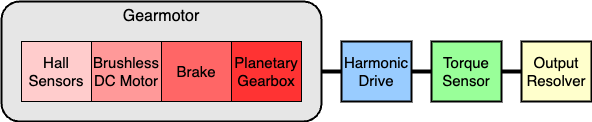
\includegraphics[width=1\columnwidth]{images/actuator_structure.png}
\caption{Hardware structure of the actuators comprising the Sample Transfer Arm. The components in the ``Gearmotor" box are in one physical enclosure.}
\label{fig:actuator_structure}
\end{figure}

\label{sec:intro}
%%%%%%%%%%%%%%%%%%%%%%%%%%%%%%%%%%%%%%
\section{Background and Related Work} 
%%%%%%%%%%%%%%%%%%%%%%%%%%%%%%%%%%%%%%


When developing a robotic system for a mission like Mars Sample Return (MSR), one of the most critical questions is whether it can deliver the desired functionality robustly and reliably. Ideally, this would be evaluated by testing the actual system in its target environment. However, during development, this is often impractical. This is particularly true in early stages, when the system doesn't yet exist, but can also apply later, when replicating mission environments is infeasible (e.g., deep-space conditions).

The value of a model depends on how faithfully it captures the true system’s behavior—its fidelity—because engineering decisions are only as reliable as the behaviors the model predicts. Early in concept studies, coarse models can rank architectures, but as requirements harden and the design is baselined, tolerances shrink and verification increasingly relies on model predictions; at that stage, a low-fidelity model risks both over- and under-estimation of performance. Finding the balance between fidelity and overdesign is really an art, as Jean-Charles Mar{'e} notes in~\cite{mare2020practical}: “The main challenge is really to actively master the modeling activity to obtain a model having just-sufficient complexity.”

Our mission required a model that would accurately capture system performance at a time when we were far into the development process. At the point of STA model conception, the actuators' mechanical structure and the control scheme were already established. Illustrated in Figure~\ref{fig:actuator_structure}, each actuator consists of a Brushless DC Motor (BLDC), position sensors, and multiple stages of gear reduction. A high-fidelity actuator model must reflect both the ideal and non-ideal attributes of these components. These include aspects such as inertia, damping, and backlash.

Additionally, at the onset of actuator model creation, the designer of the robot arm, Leonardo (on contract from the European Space Agency (ESA)) had already established the control scheme of the existing actuators. As will be further elaborated upon later on in this paper, this control scheme was a cascaded position-velocity-current controller that closed its loops using a variety of onboard sensors. This controller primarily took position setpoints but also could take feed-forward velocity/current values.

In previous work, modeling of BLDC motors have been explored extensively with models exhibiting varying degrees of fidelity. Some, such as Krykowski et al. in~\textbf{\cite{krykowski2013constant}}, opt to create a more simplified electrical representation of the motor. While some aspects are still modeled, some that depend on rotor angle such as torque ripple are missing. Tibor et al.~\textbf{\cite{tibor2011modeling}} created a mathematical model of a BLDC motor and the three-phase H-bridge inverter used to perform six-step commutation. They were able to demonstrate realistic phase waveforms and resultant torque ripple. However, significant nonlinear components—such as static friction—were not included. In addition, many publications go no further than the motor itself, neglecting to model the control scheme—an essential component for capturing non-ideal effects in practice. Some models, such as \cite{pillay1989modeling}, include a speed controller that modulates the applied voltage via PWM to track different reference speeds. This is a step in the right direction; however, in many applications—particularly robotic systems where users specify desired arm configurations—position control is paramount.

Other models include both a BLDC motor and a position controller. Vedadi et al. accomplish this by using cascaded position and speed control loops~\textbf{\cite{vedadi2025optimized, vedadi2021optimized}}. Yet the fidelity of the BLDC motor is compromised, as the dynamics are approximated in a purely linear state-space representation. Additionally, ideal position and velocity feedback are assumed. Similarly, Manoharan et al. use a cascade controller but do not assume ideal feedback, introducing white noise into the speed measurement~\textbf{\cite{manoharan2024cascade}}. However, their system model incorporates the Simscape BLDC motor block, which has only an intermediate level of fidelity~\textbf{\cite{mathworks2025bldc}}.

%%%%%%%%%%%%%%%%%%%%%%%%%%%%%%%%%%%%%%
\section{Model Structure} 
%%%%%%%%%%%%%%%%%%%%%%%%%%%%%%%%%%%%%%

\subsection{High-Level Structure}
Most control systems can be boiled down into three parts: the plant, the controller, and the feedback. Motor control exemplifies this paradigm. Admittedly, there is some ambiguity on where the lines are drawn but at a high level, the motor dynamics, the motor controller, and the sensor feedback correspond to the plant, the controller, and the feedback (Figure~\ref{fig:high_level_control_system}).
\begin{figure}[!htb]
\centering
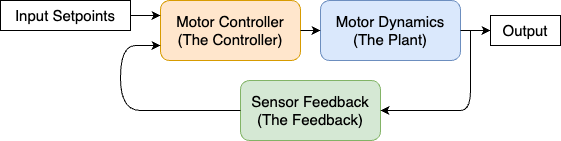
\includegraphics[width=1\columnwidth]{images/high_level_control_system.png}
\caption{High-level diagram of the general motor control paradigm.}
\label{fig:high_level_control_system}
\end{figure}
\subsection{Motor Dynamics}
The dynamics of our motor model can be broken down into three states: the electromechanical stage (the junction between the electrical and mechanical part of the motor), the motor stage (the mechanical dynamics of the motor), and the output stage. The electromechanical stage can be described as the junction where electrical power is converted to mechanical power. Mathematically, this relationship is 
\begin{align*}
\tau_{\text{mech}}(i_q,\theta_m)=k_ti_{q}-\tau_{\text{cogging}}(\theta_m)
\end{align*}
where $i_q$ is the active current, the component of the total current that produces a stator magnetic field orthogonal to the rotor magnetic field, and $k_t$ is the torque constant defining the motor-specific current-to-torque relationship. $\tau_{\text{cogging}}(\theta_m)$ reflects torque that results from magnetic interactions between the stator slots and the permanent magnets on the rotor--interactions that are present with or without energizing the stator coils.

The mechanical torque $\tau_{\text{mech}}$ drives the motion of the motor stage, as shown on the left side of Figure~\ref{fig:torsional_stiffness}. We use the equation for Stribeck friction presented in ~\textbf{\cite{armstrong1994survey}}
\begin{align*}
\tau_{f}(\dot{\theta}_m)&=\mu_k\text{sign}(\dot{\theta}_m),\;\;\tau_{s}(\dot{\theta}_m)=\mu_s\text{sign}(\dot{\theta}_m)\\
\tau_{\text{friction}}(\dot{\theta}_m)&=\tau_{f}+(\tau_{s}-\tau_{f})\exp\left(-\alpha_{s}|\dot{\theta}_m|\right)+B_m\dot{\theta}_m
\end{align*}
to yield a relationship between mechanical torque, the rotor's motion, and the torque delivered to the beginning of the output shaft $\tau_{\text{in}}$:
\begin{align*}
\tau_{\text{mech}}(i_q,\theta_m) &= J_m\ddot{\theta}_m + \tau_{\text{friction}}(\dot{\theta}_m) + \frac{1}{g_r}\tau_{\text{in}}
\end{align*}
Where $g_r$ is the gear ratio of the gearbox. To compute the torque transmitted through the output shaft, we model the shaft and gearbox as a torsional spring-damper system. This model accounts for torsional stiffness and damping as well as backlash, as illustrated in Figure~\ref{fig:torsional_stiffness}. Typically, torsional stiffness is given as $\tau_{\text{out}}=-\tau_{\text{in}}=K_{\text{stiff}}\Delta\theta+B_{\text{stiff}}\Delta\dot{\theta}$ where $K_{\text{stiff}}$ and $B_{\text{stiff}}$ are the torsional stiffness and damping coefficients, respectively. However, due to the presence of backlash in the planetary gearbox (see inset in Figure~\ref{fig:torsional_stiffness}), we modify the standard torque transmission model to include a deadband.

Specifically, the torque transmitted through the spring-damper is zero when the angular displacement remains within the backlash gap $\delta$:
\begin{align*}
\Delta\theta&=\frac{1}{g_r}\theta_m-\theta_{o}, \;\;\Delta\dot{\theta}=\frac{1}{g_r}\dot{\theta}_m-\dot{\theta}_o\\
\tau_{\text{stiff}}&=K_{\text{stiff}}(\Delta\theta-\delta\text{sign}(\Delta\theta))+B_{\text{stiff}}\Delta\dot{\theta}
\end{align*}
\begin{align*}
\tau_{\text{out}}=\begin{cases}
  \tau_{\text{stiff}}, & |\Delta\theta| > \delta \\
  0, & \text{else}
  \end{cases}
\end{align*}
Finally, we incorporate the output shaft dynamics, which include its inertia and damping, as well as any externally applied torques:
\begin{align*}
\tau_{\text{ext}}=\tau_{\text{out}}-J_o\ddot{\theta}_o-B_o\dot{\theta}_o
\end{align*}
\begin{figure}[!b]
\centering
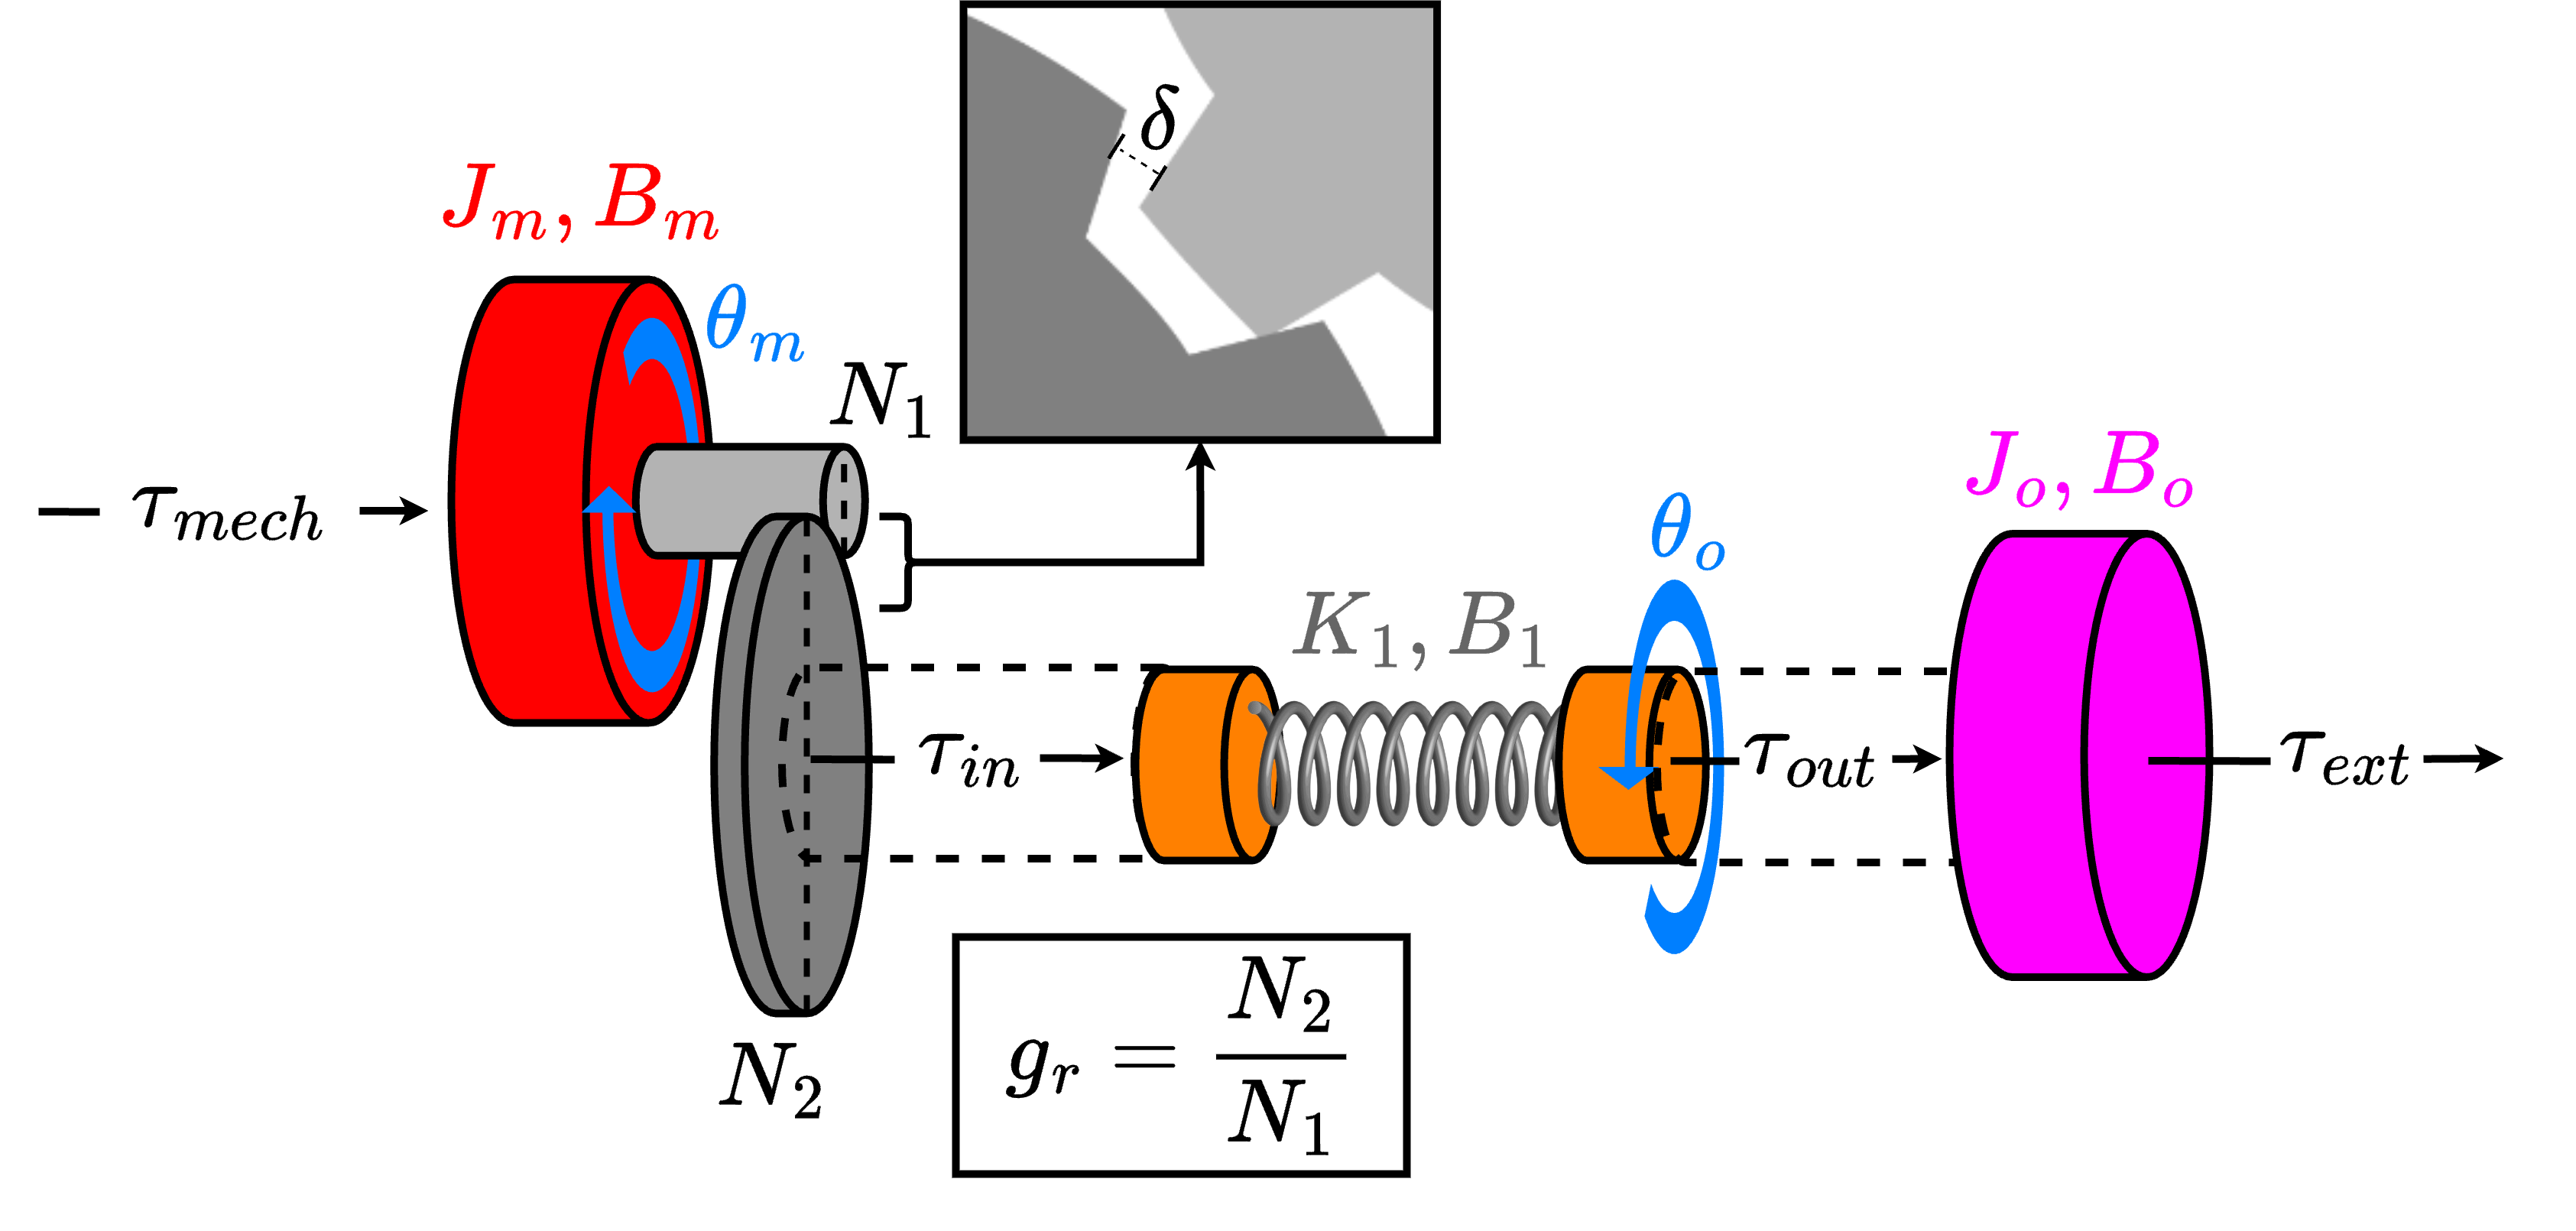
\includegraphics[width=1\columnwidth]{images/torsional_stiffness.png}
\caption{Illustration of torsional stiffness for a motor, gearbox, and output shaft.}
\label{fig:torsional_stiffness}
\end{figure}
Manufacturer datasheets provide most electromechanical parameters (e.g., $J_m$, $J_o$, $k_t$, $g_r$, $\delta$), but internal damping coefficients ($B_m$, $B_o$) are typically unspecified. In this work, we choose damping so that the simulated actuator intentionally underperforms measured hardware over the exercised band. This mission-conservative choice avoids overstating capability.

\subsection{Motor Controller}
The motor controller’s role is to supply the appropriate amount of active current to achieve a desired objective. In our case, the objective is to reach position setpoints with minimal delay. Since different robotic arm configurations can lead to varying external torques, the controllers must maintain accurate position tracking across a range of torque loads.
For technical reasons such as strong disturbance rejection~\cite{vedadi2025optimized}, Leonardo uses a cascaded position-velocity-current controller (Figure~\ref{fig:cascade_controller}).
In this cascade, inner loops operate at progressively higher bandwidths. With typical tuning yielding a current loop bandwidth an order of magnitude or more above the outer loops, it is common practice to approximate the current loop as unity gain (i.e., an ideal torque source)~\textbf{\cite{parker_servo_fundamentals}}. Accordingly, we model the current loop so that setpoints from the velocity controller produce instantaneous active current ($i_q\gets i_q^{\text{(sat)}}$). 
For the velocity and position loops, we use a PI controller and a P controller, respectively. Current saturation enforces output limits, and back-calculation anti-windup mitigates integrator windup (Figure~\ref{fig:pos_vel_controller}).
% Talk about the math for each component of the controller and the non-linearities
\begin{figure}[!htb]
\centering
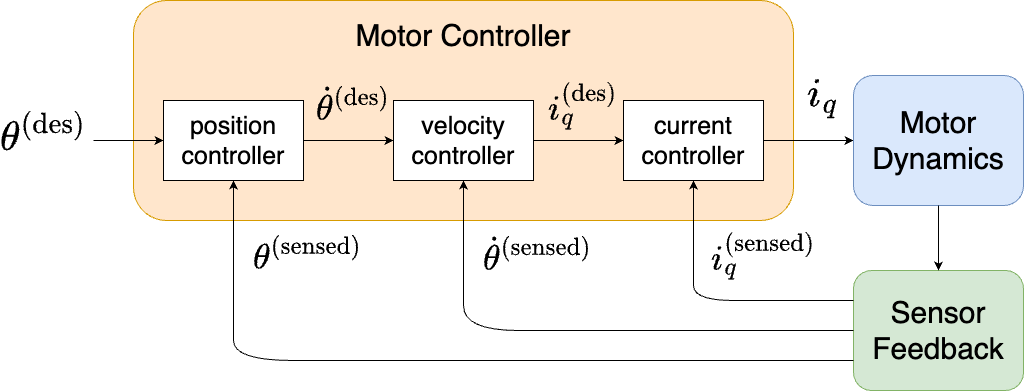
\includegraphics[width=1\columnwidth]{images/cascade_controller.png}
\caption{Cascade controller construction used for the Sample Transfer Arm actuators.}
\label{fig:cascade_controller}
\end{figure}
\subsection{Sensor Feedback}
The internal control loops of the cascade controller rely on actuator state measurements captured by real sensors. These sensors are not free of imperfections and, if the controller is not robust enough, these imperfections can impact the overall performance of the actuator. Consequently, it is essential that highly impactful issues are addressed. 

To measure the speed of the rotor, the Sample Transfer Arm employs three Hall Effect sensors. As the rotor rotates and permanent magnets interact with these sensors, six total transitions occur per electrical cycle. The velocity $\dot{\theta}_m$ is then determined by measuring the time difference between subsequent transitions. Ideally, each transition accounts for 60 degrees of electrical cycle. However, this requires accurate placement preserving 120 electrical degree separation between halls. A hall sensor misplacement of only a few mechanical degrees corresponds to a much larger electrical misplacement, since the electrical angle scales with the number of poles $P$ (Figure~\ref{fig:hall_sensor_misplacement}). Alaeinovin et al.~\textbf{\cite{alaeinovin2008evaluating}} provide the relation between mechanical angle $\phi_{mx}$ and electrical angle $\phi_{x}$ as $\phi_{x}=\frac{P}{2}\phi_{mx}$.

To approximate the resulting error due to mechanical misplacement, we assume that the misplacement of each Hall sensor is drawn from a normal distribution with zero mean and a chosen standard deviation $\sigma$. This leads to the following measurement error in electrical angular velocity $\theta_e$ when calculated at a Hall state transition:
\begin{align*}
&\phi_x\sim {\mathcal{N}}(0, \sigma^{2}),\quad \text{where }x\in\{A,B,C\} \\
&\Delta \phi_e = \SI{60}{\degree} + \phi_{x,\text{curr}} - \phi_{x,\text{prev}}\\
&\Delta t = t_{\text{curr}} - t_{\text{prev}} \\
 &\dot{\theta}_e = \frac{\Delta \phi_e}{\Delta t} \\
\therefore\quad &e = \dot{\theta}_e^{\text{ideal}} - \dot{\theta}_e = -\frac{\phi_{x,\text{curr}} - \phi_{x,\text{prev}}}{\Delta t}
\end{align*}
From this, we observe that misplacing one Hall sensor produces two erroneous velocity estimates, since two Hall transitions in each electrical cycle depend on its position. Therefore, the six velocity estimate errors observed over a full cycle are not statistically independent. In fact, these errors are linear combinations of only three independent random variables—the mechanical misplacements of the Hall sensors—which induces statistical correlation between errors at different transitions.

However, for implementation simplicity and to ensure robustness to additional sources of randomness, we choose to model each transition error as independent. We further assume that the sensed rotor velocity is the true velocity plus the error associated with a randomly selected Hall transition:
\begin{align*}
e_i \sim {\mathcal{N}}(0, \sigma^{2}), \quad i \in {1, \dots, 6} \\
\dot{\theta}^{\text{(sensed)}}[n] = \dot{\theta}[n] + e_k, \quad k \sim {\mathcal{U}}\{1,6\}
\end{align*}
The implementation of the resolver measurement can be modeled as a moving average filter of length four applied to the true angle signal corrupted by additive Gaussian noise. Formally,
\begin{align*}
\theta^{(\text{sensed})}[n]=\frac{1}{4}\sum_{k=1}^{4}\left(\theta[n-k]+v_k\right),\quad v_k\sim{\mathcal{N}}(0,\sigma_{\text{resolver}})
\end{align*}
where $\theta[n-k]$ is the true angle at time $n-k$, and $v_k$ are independent Gaussian noise samples representing resolver measurement noise.
\begin{figure}[!htb]
\centering
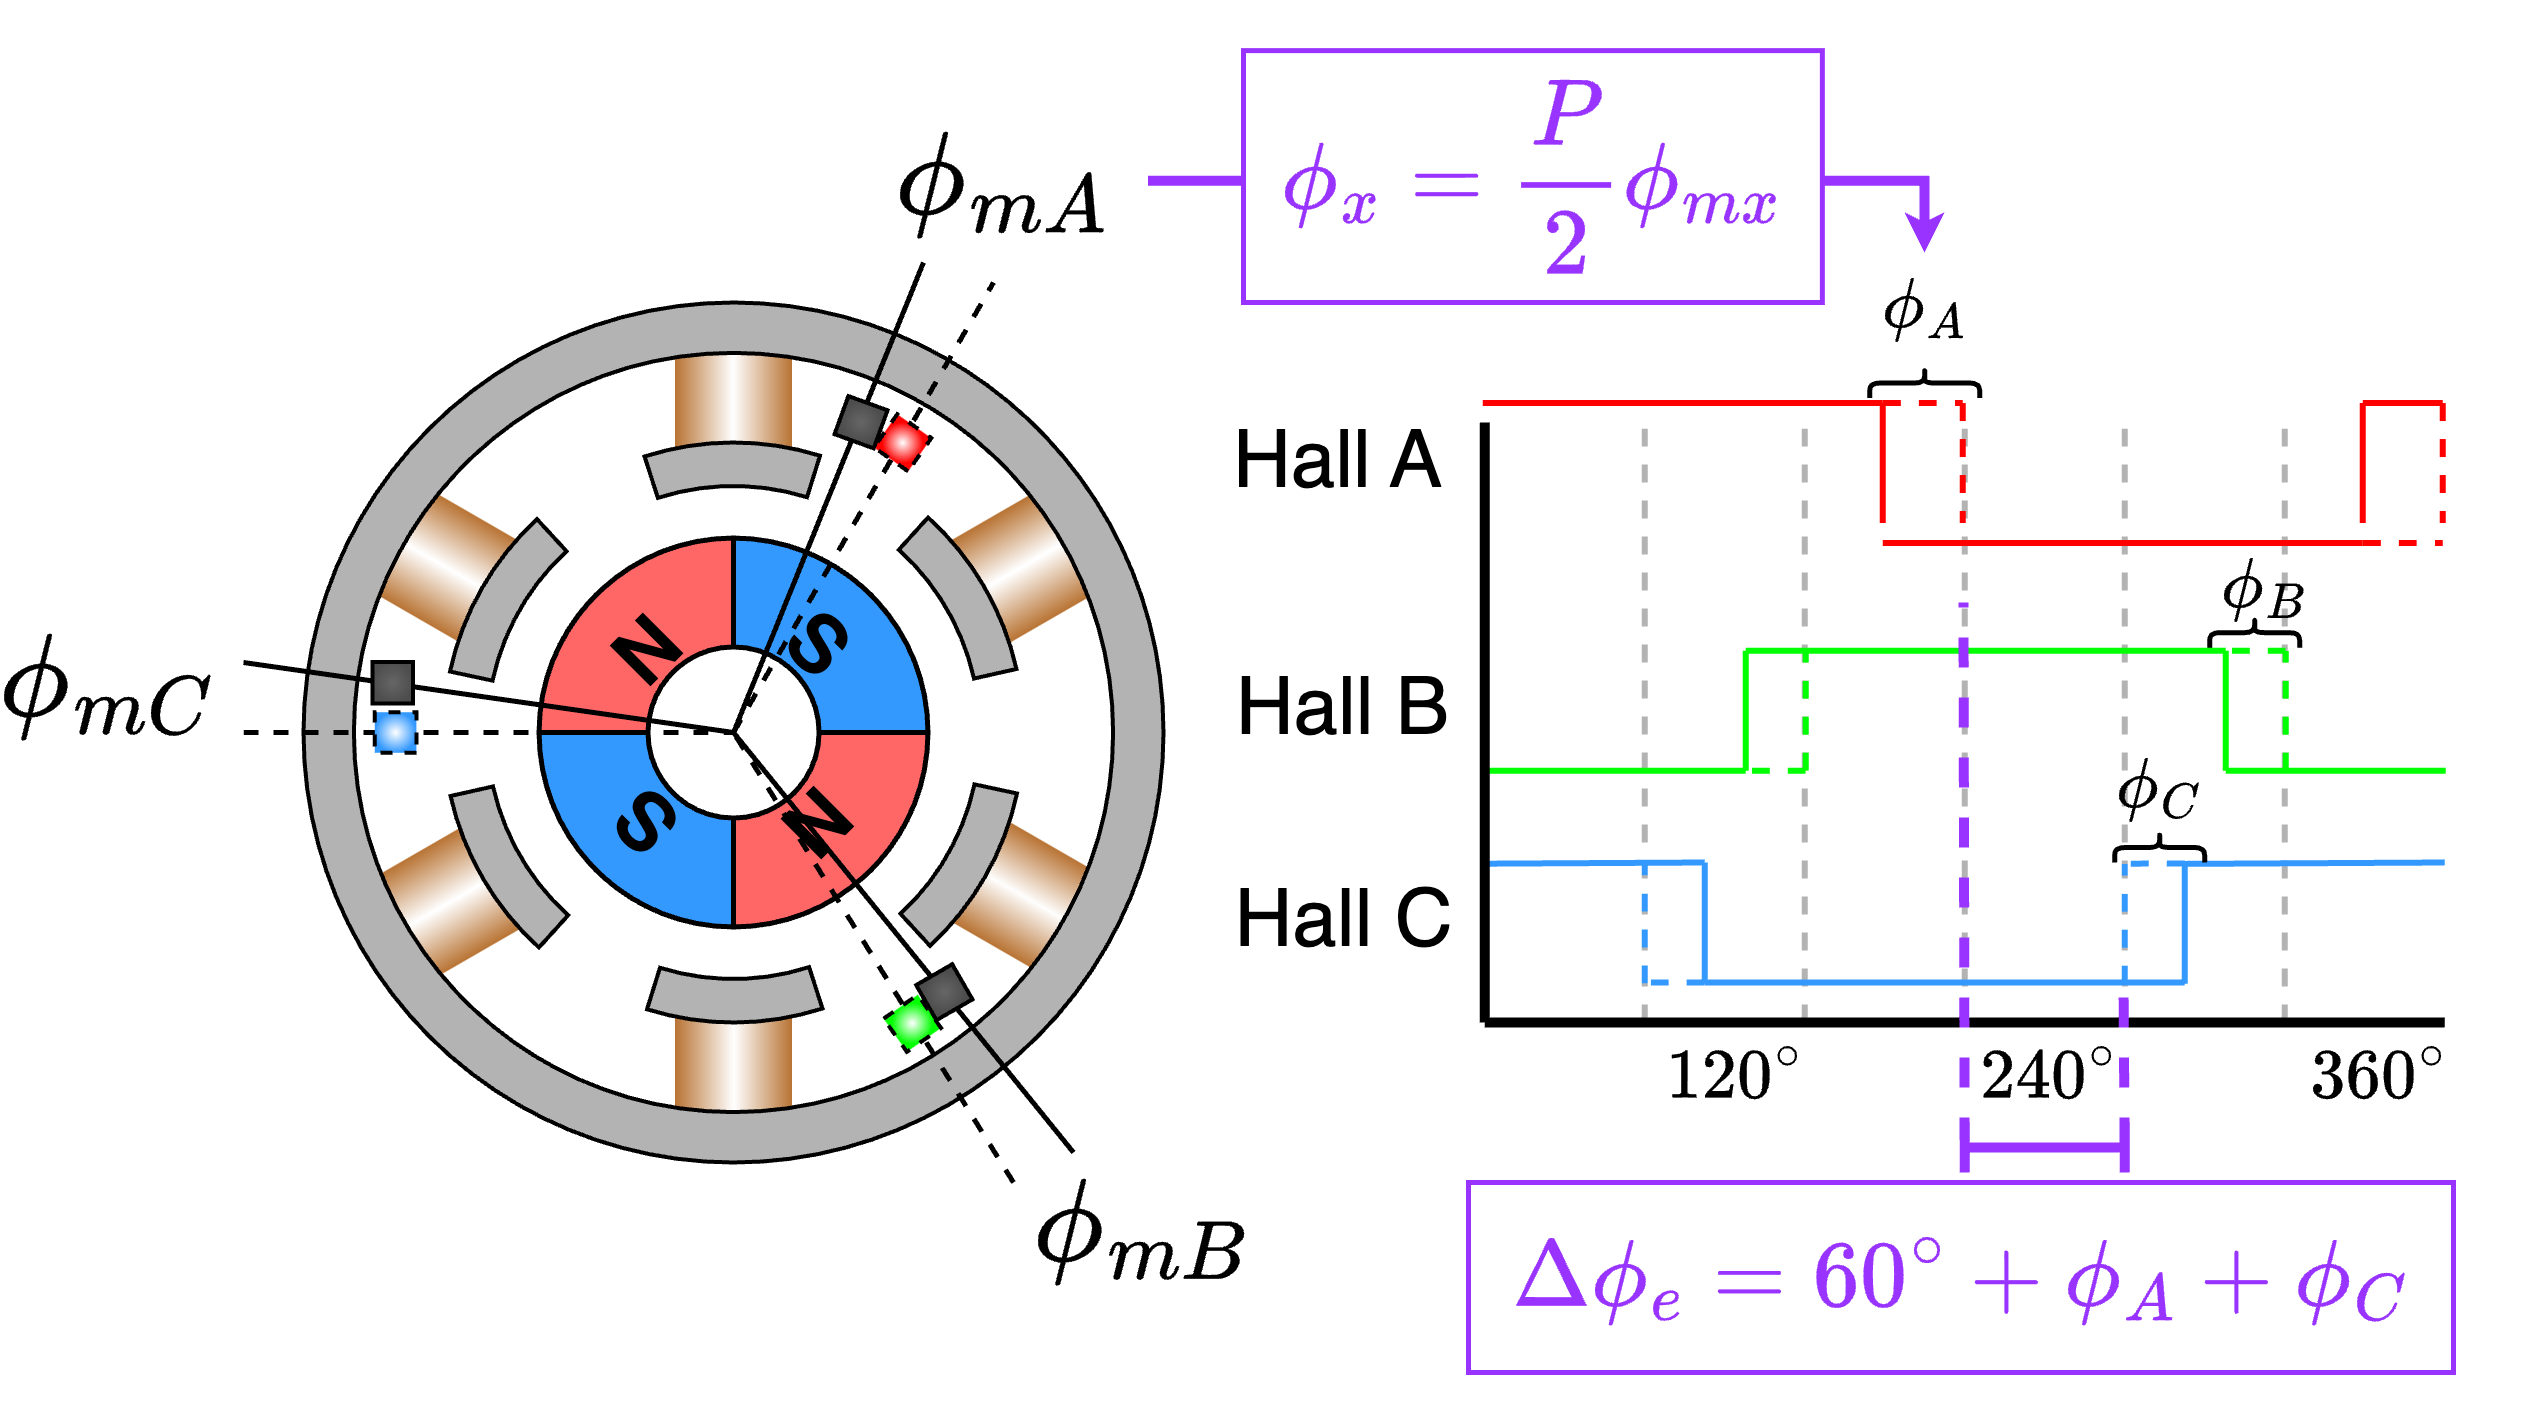
\includegraphics[width=1\columnwidth]{images/hall_sensor_misplacement.png}
\caption{Impact of mechanical misplacement on angular velocity estimation.}
\label{fig:hall_sensor_misplacement}
\end{figure}

\newpage
\begin{figure*}[!t]
\centering
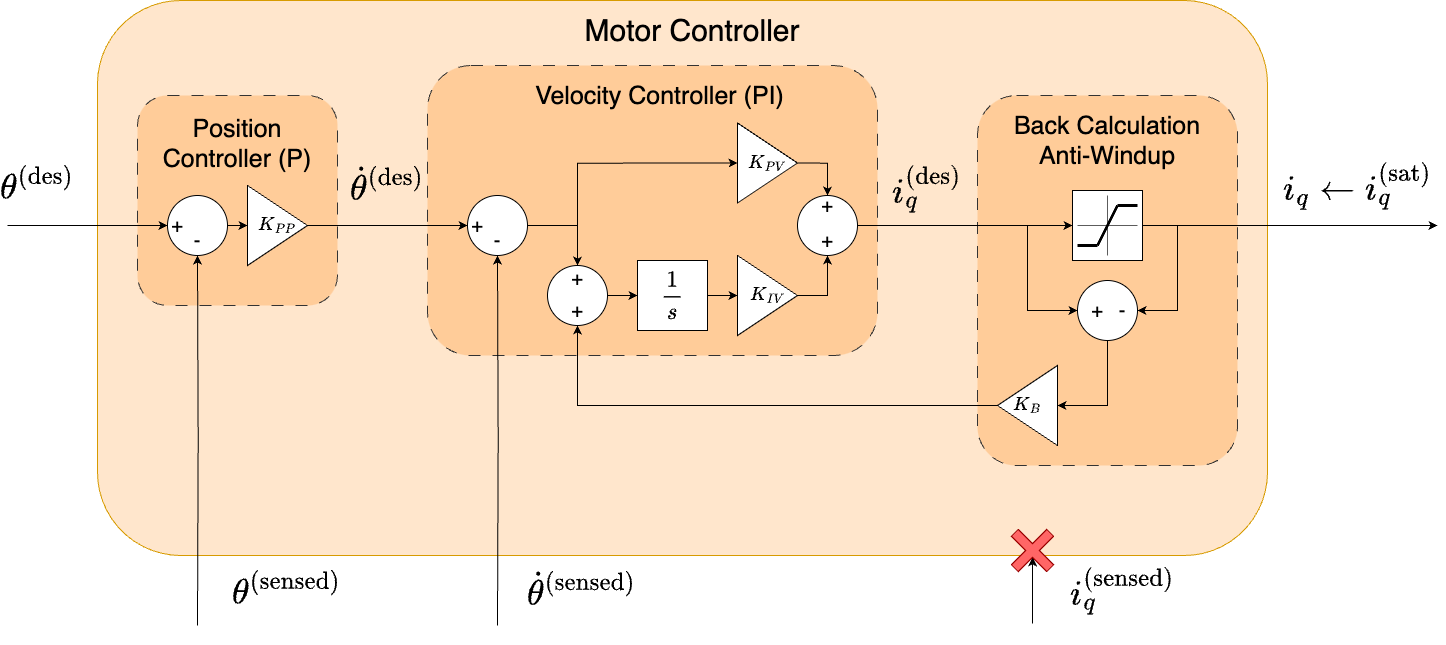
\includegraphics[width=\textwidth]{images/pos_vel_controller.png}
\caption{Modeled cascade controller incorporating back calculation anti-windup. The current loop is not modeled because it operates at a significantly higher frequency than the outermost position loop.}
\label{fig:pos_vel_controller}
\end{figure*}

\section{Usage}
A primary goal during the development of this actuator model is to ensure this model is project-agnostic meaning other projects could easily integrate this model into their design process. We identify two key features as necessary for this: modularity and parameterization.

\subsection{Modularity}
Too often, Simulink models are built without proper modularization, making it difficult for users to understand and work with individual components. This lack of structure becomes especially problematic when part of the model needs to be replaced or updated. In robotics, where system requirements frequently shift, such changes are common. For example, actuator subsystems may require swapping out a controller or altering the method of state observation. As emphasized in~\textbf{\cite{whalen2014structuring}}, a change to a single requirement should not have an undue impact on unrelated parts of the model or on the verification artifacts used to validate it — underscoring the importance of modularity to localize changes and simplify ongoing model maintenance.




For modularity, we separate the actuator model into three sub-models that are used via Simulink's ModelReference block. Pictured in Figure~\ref{fig:simulink_model}, we observe that, at a high-level, this structure is identical to the general motor control paradigm shown in Figure~\ref{fig:high_level_control_system}. This structure explicitly conveys the role of sub-modules facilitating component-wise modification.

\subsection{Parameterization}
\label{sec:parameterization}

As alluded to in the ``Background and Related Work" section, the mechanical makeup of the actuators on the SRL STA is fixed at the time of actuator model conception. However, the arm was not fully constructed nor available at that time. As such, we have constructed robotic arm testbeds that are topologically equivalent to the true SRL Sample Transfer Arm. ``Topologically equivalent" meaning that each robotic arm, and its embedded actuators, could be described by the same list of parameter values.
Such a choice is conducive to describing each actuator in terms of parameter files with equivalent fields. For this purpose, we use the YAML file format given its widespread use and pre-existing MATLAB libraries.

Care was taken when deciding how many parameter files, and the corresponding content, were used per actuator. Going along with the theme of increased modularity, three total parameter files were used to describe each actuator: the controller file, the physical file, and the toggles file. As their names suggest, the controller and physical parameter files are used to describe the controller sub-model and the physical dynamics sub-model. Notably, a distinct file for the feedback sub-model could not be constructed as the performance of feedback components depends on both controller and physical parameters (e.g., the dependency of the speed sensor on the number of hall sensors as well as the controller period). Lastly, the toggles parameter file is used to enable or disable nonlinear components of the actuator model thereby allowing a trade-off between model accuracy and computation cost. As with real-life actuators, minor differences in actuator YAML files may yield significant changes in model results (as illustrated in Figure~\ref{fig:yaml_ingestion}).

\clearpage 
\onecolumn

\begin{figure*}[!t]
\centering
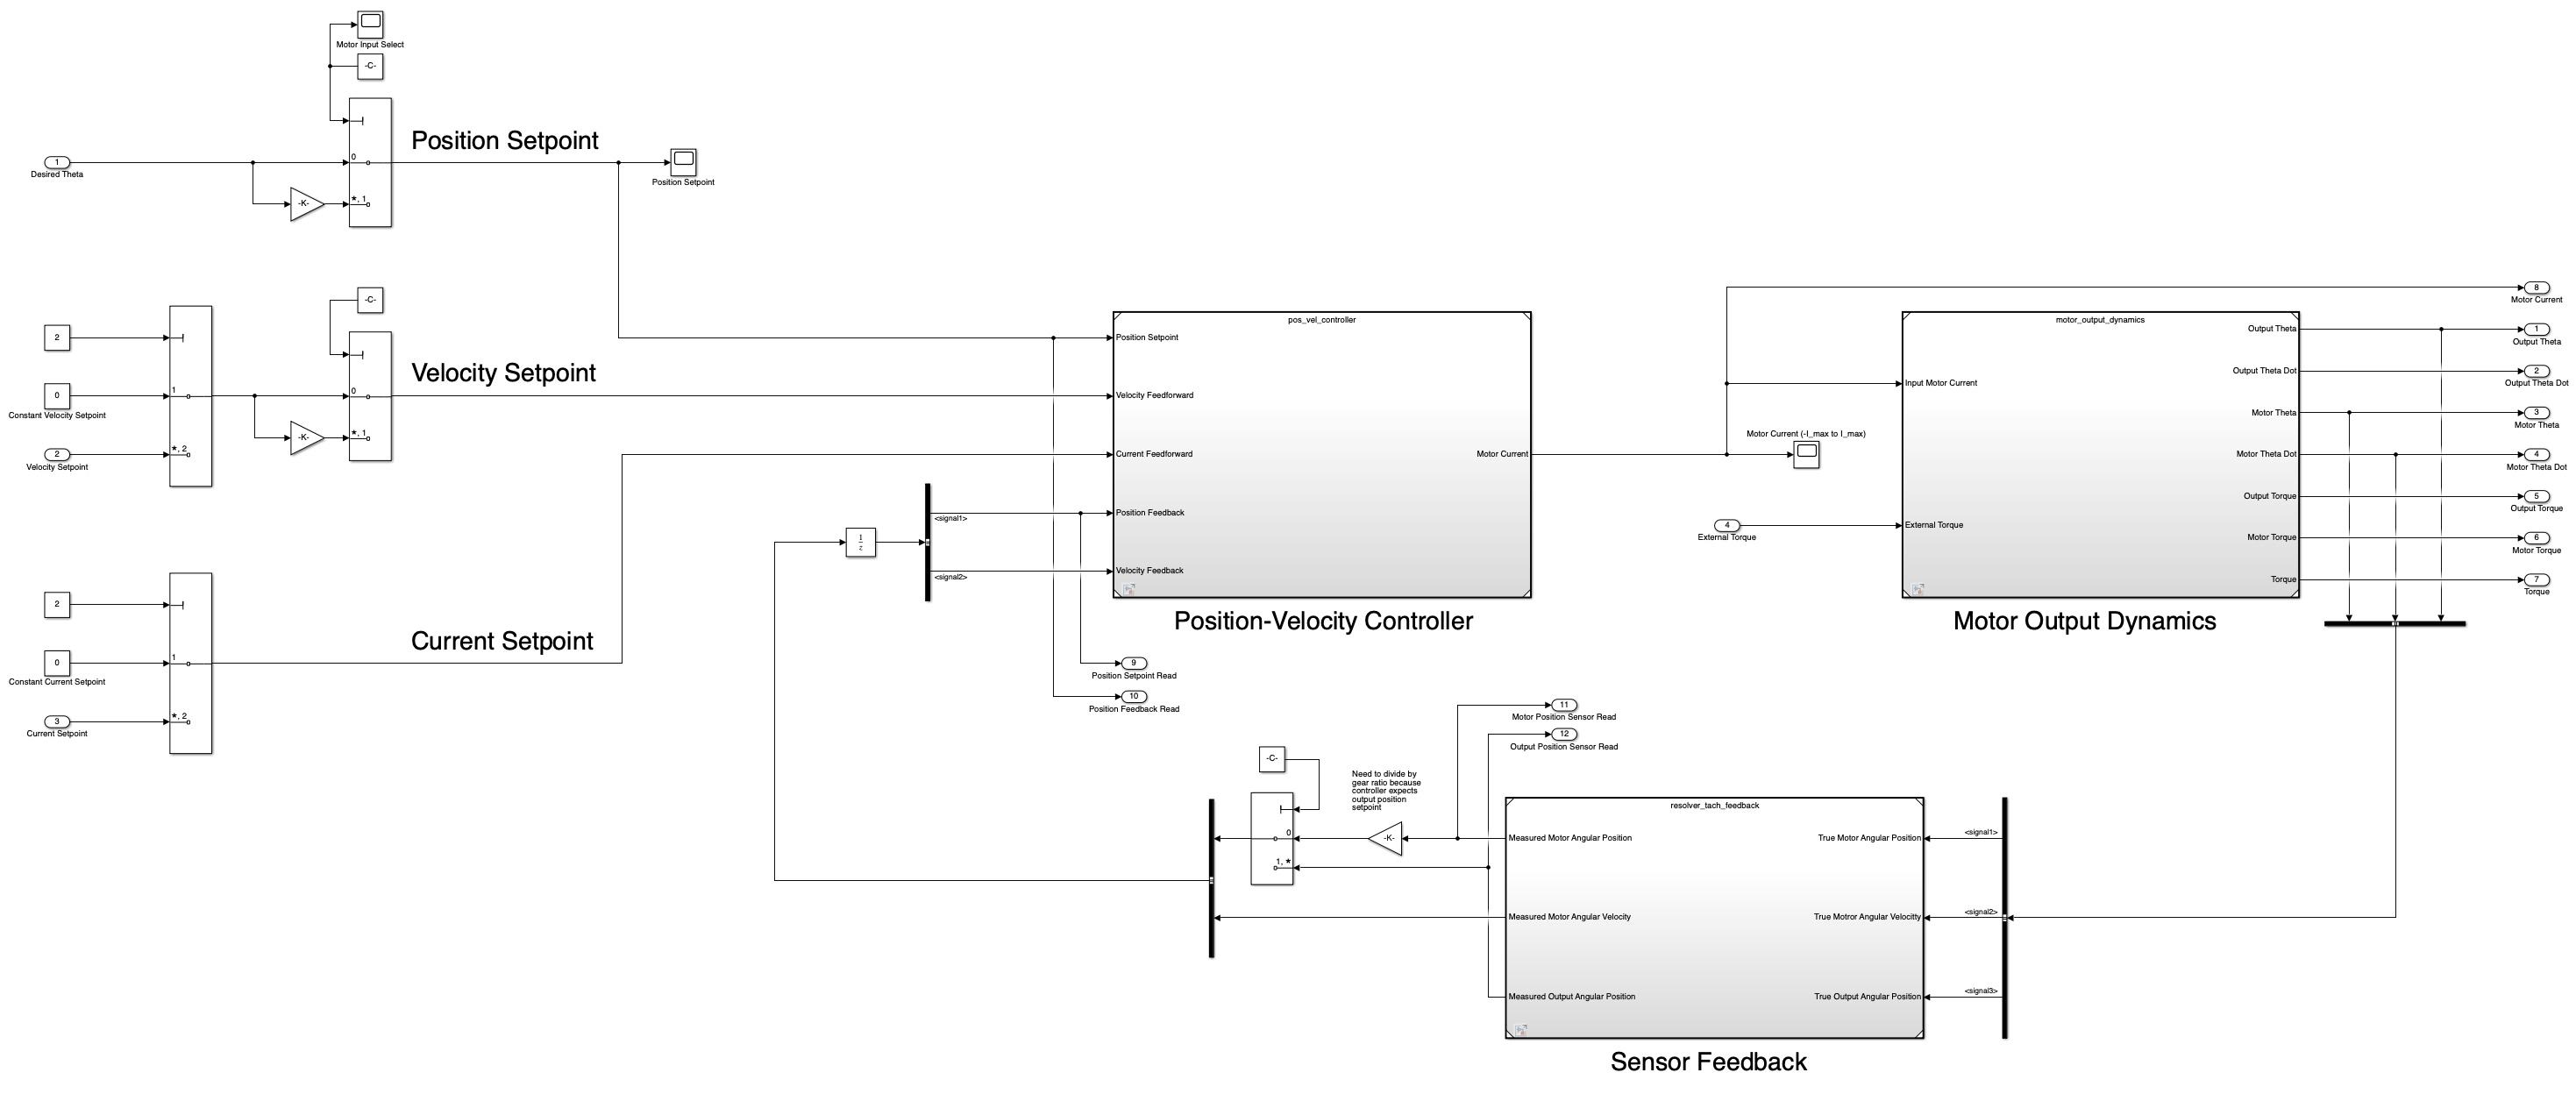
\includegraphics[width=\textwidth]{images/simulink_model.jpeg}
\caption{Structure of the actuator model in Simulink.}
\label{fig:simulink_model}
\end{figure*}


\begin{figure*}[!b]
\centering
\includesvg[width=1\textwidth]{images/yaml_ingestion.svg}
\caption{Illustration of the impact of YAML parameter files on actuator model behavior. Modifying parameter values within these files alters model performance, potentially resulting in differing output responses to identical input position waveforms.}
\label{fig:yaml_ingestion}
\end{figure*}


\clearpage 
\twocolumn
\subsection{Landing Gear Simplified Example}

To demonstrate the benefits of a high-fidelity actuator model beyond space robotics, we draw inspiration from current trends in aviation research, particularly efforts toward the More-Electric Aircraft (MEA) concept. This approach emphasizes replacing traditional hydraulic actuators with electromechanical actuators (EMAs) to reduce weight and improve efficiency. For small aircraft such as Unmanned Aerial Vehicles (UAVs), minimizing weight is critical, and using EMAs instead of hydraulic actuators can yield significant weight savings~\textbf{\cite{botten2000flight}}.

Typical aircraft landing gear construction includes two actuators: a main actuator and a locking actuator. The main actuator functions to extend the landing gear and consequently experiences high loads during operation. Once the landing gear is near full extension, the locking actuator secures it in the extended position. This locking action prevents continuous loading on the main actuator by transferring the high loads experienced during aircraft touchdown to the mechanical locking components of the landing gear.

We create a simplified example of a typical landing gear with two actuators in MATLAB using both standard Simulink and Simscape components.  The actuator model described in this paper is used for both actuators, each configured with different sets of YAML parameter files. The most notable difference between them is the gear ratio, which is adjusted to reflect the increased output torque requirements of the main actuator. By modeling the mechanical components of the landing gear with Simscape bodies and joints, we obtain the torque demands of the system on the two actuators. These torque demands are fed into the actuator model as external torques as shown in Figure~\ref{fig:aelg_control_diagram}.
\begin{figure}[!b]
\centering
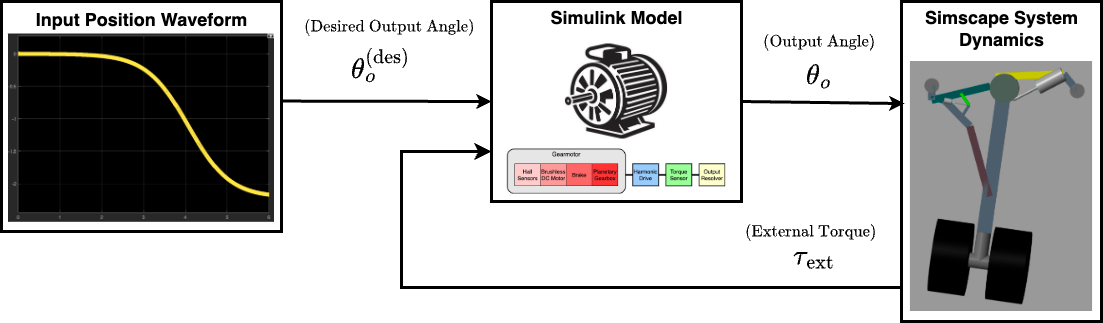
\includegraphics[width=1\columnwidth]{images/aelg_control_diagram.png}
\caption{High-level control diagram for the simulated landing gear system. Desired input angle waveforms are fed into the actuator model, the output of which is fed into a dynamics model of a plane landing gear linkage system, and the torque necessary to reach this output is fed back into the actuator model as external torque.}
\label{fig:aelg_control_diagram}
\end{figure}
This landing gear system demonstrates how the high-fidelity actuator model can be applied to system design beyond robotic arms for space applications. To assess whether the main and locking actuators, as defined in the parameter files, are suitable for this application, we evaluate actuator performance during the initial extension of the landing gear and the locking of mechanical components.

As an example, Figure~\ref{fig:aelg_primary_motion} shows the main actuator’s performance during the initial extension phase—referred to as the ``primary motion." From these plots, we observe a peak tracking error of \SI{0.4}{\radian}, which occurs when the input waveform demands the highest output angular velocity. Results like these enable system designers to assess whether such errors are acceptable and identify potential actions to improve performance.

\begin{figure}[!htb]
\centering
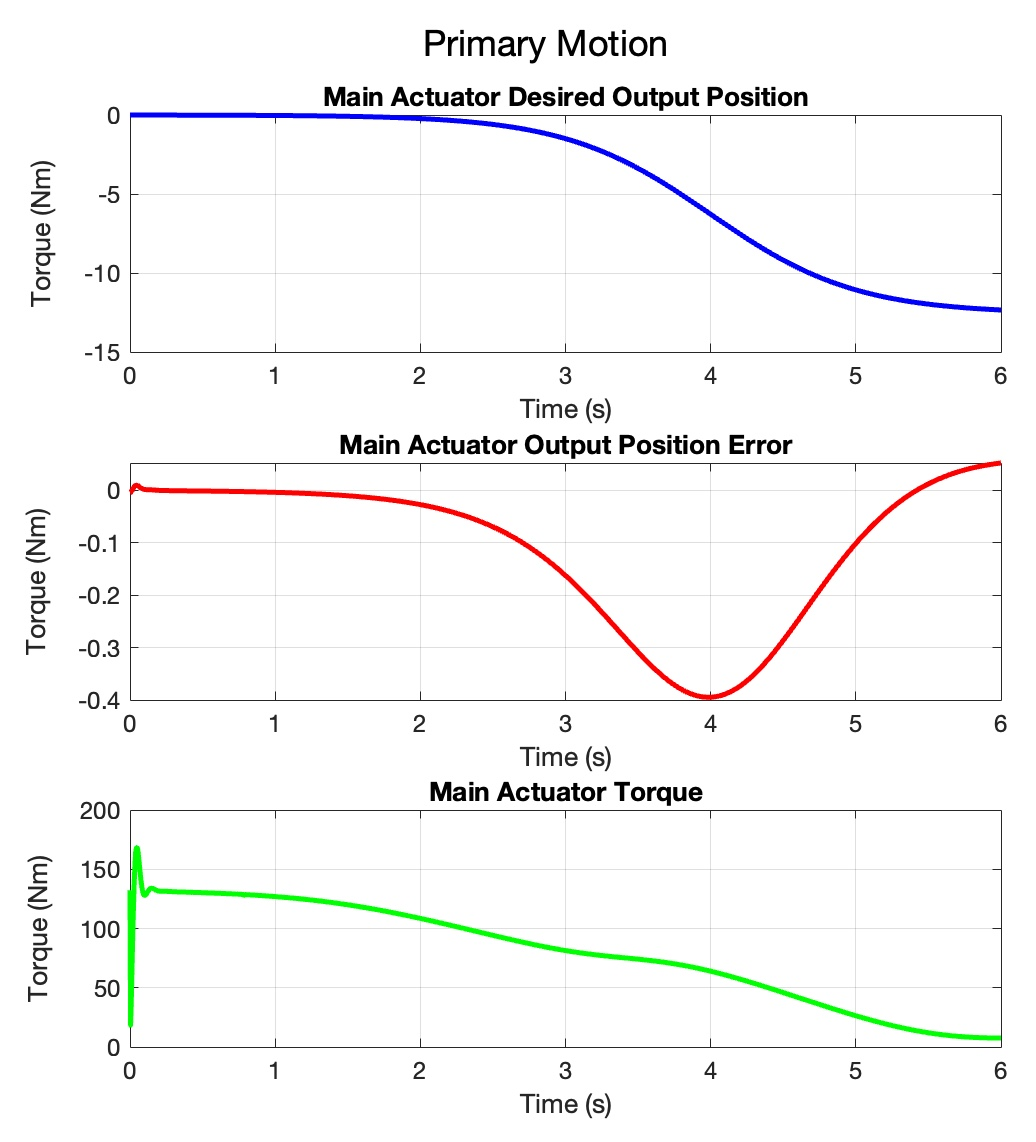
\includegraphics[width=1\columnwidth]{images/aelg_primary_motion.jpeg}
\caption{Output position error (red) and actuator torque (green) during the primary motion of the landing gear system. The maximum position error occurs when the desired output angular velocity is highest (blue curve, steepest slope). The torque plot shows that the main actuator requires at most \SI{175}{N\,m} during this motion.}
\label{fig:aelg_primary_motion}
\end{figure}

\subsection{Adapting the Model to New Applications}

Porting the actuator model to a new application primarily affects the choice of controller implementation and parameter files rather than the high-level structure. Aside from possible changes to the drive controller architecture (which are localized to the controller sub-model), new use cases typically require updated YAML files reflecting differences in the actuator’s electromechanical characteristics (e.g., gear ratio, torque constant, inertias). Because actuator assembly is not perfectly repeatable, even mechanically equivalent units generally require some re-identification, particularly in controller tuning and damping coefficients.

\begin{figure*}[!htb]
\centering
\includesvg[width=\textwidth]{images/actuator_bode_plots.svg}
\caption{Bode plots comparing three real actuators (in red) versus their simulated counterparts (linear model in blue and nonlinear model in pink). The first, second, and third columns correspond to the bode plots for Actuator 1, Actuator, 2, and Actuator 3, respectively.}
\label{fig:bode_plots}
\end{figure*}

\newpage 
\section{Model Validation}
We compared model performance to real actuator performance to validate the model. We chose Bode plots because they permit the use of well-understood, classical control methods of analysis—stability margins, resonant frequencies, etc. Additionally, one can easily view performance throughout a frequency range. Using these analysis tools, we wanted to ensure the actuator model had similar performance yet did not outperform the real actuator.

\subsection{Equipment}
Three actuators were constructed that abide by the mechanical structure shown in Figure~\ref{fig:actuator_structure}. Each actuator varied parametrically with differences in gear ratio, inertia, damping, etc. Power was supplied to the motor windings via ELMO Gold Drivers. Internally, the ELMO Gold Drivers implement a cascade controller with the same high-level construction of Figure~\ref{fig:cascade_controller}. Each loop in the cascade controller was then tuned sequentially starting from the inner-most current control loop to the outer-most position control loop. Tuning was done to ensure a desired closed-loop bandwidth using the Expert Tuning tool within the Elmo Application Studio software.

\subsection{Testing Method}
We then constructed Bode plots for the real actuators. Construction involved applying sinusoidal waveforms as input waveforms and recording the resulting output waveforms in simulation and in real life. These input waveforms were of equivalent amplitude but differing frequency. Next, we calculated the amplitude and phase difference between the input and output waveforms. Each difference in amplitude and phase accounted for one data-point on the magnitude and phase plot, respectively.

The three actuators were described using YAML parameter files, as detailed in Section~\ref{sec:parameterization}. These YAML files described the physical attributes and the control loop gains found during the controller tuning. These files were then used to simulate the three actuators in two model configurations: all nonlinearities turned off and all turned on. Using the same input waveforms as in the real-life tests, Bode plots were constructed for these simulated actuators. A juxtaposition of the real-life actuator Bode plots and the simulated actuator Bode plots was shown in Figure~\ref{fig:bode_plots}.

\subsection{Analysis}
From these plots, for all three actuator types the linear and nonlinear models underpredict the true actuator’s bandwidth. Moreover, with nonlinearities enabled the model’s magnitude response is strictly lower than the linear model at every measured frequency $\Omega_{\text{test}}$—i.e.,
\begin{equation}
  |G_{\mathrm{NL}}(j\omega)| < |G_{\mathrm{LIN}}(j\omega)|,\;\; \forall \omega \in \Omega_{\text{test}},
\end{equation}
which is consistent with the added dissipative effects we model (Stribeck friction). 

Unlike the simulation results, the hardware tests exhibit a resonance at approximately $3\,\text{Hz}$ for both Actuator~1 and Actuator~2. We attribute this $\sim 3\,\text{Hz}$ feature to dynamics not captured by the current model, including torsional compliance within the gear train (e.g., between the gearbox and harmonic drive) and small structural flex in the test fixture.

Within the tested frequency range, two actuator configurations do not exhibit a \SI{0}{\decibel} magnitude crossover in the model responses, and none of the phase traces reach \SI{-180}{\degree}, so classical gain/phase margins cannot be read directly from these plots.




\section{Limitations and Future Work}
The results presented here are limited by the frequency range over which experiments were conducted. Testing was restricted to the nominal operating band of the SRL STA actuators, which precluded full characterization of higher-frequency dynamics (e.g., high-order resonances). In addition, because several actuator configurations did not exhibit a unity-gain crossover and none reached $-180^\circ$ phase within the tested bandwidth, classical gain and phase margins could not be directly calculated, limiting the ability to make quantitative robustness comparisons between models and hardware.

Another fidelity limitation is our treatment of sensor and drive timing. In the real system, position and velocity feedback to the cascaded controller pass through the commercial ELMO firmware, which introduces time-varying transport delay and jitter. In the model, these effects are approximated with a fixed transport delay. Incorporating a more realistic representation of timing jitter would improve fidelity and better reflect the robustness of the cascaded controller to such delays; however, because the controller software is proprietary and provided as a black box, we were unable to directly characterize these timing effects for modeling purposes.

Future work will expand the tested frequency range to enable calculation of loop-shaping metrics and expose high-frequency asymmetries between simulation and reality. In addition, damping parameters were conservatively tuned in this study to ensure the model underperforms relative to hardware. To address this limitation, dedicated experiments will be conducted to identify damping coefficients ($B_o$, $B_m$) directly, enabling a more accurate comparison. We also intend to repeat the characterization process on actuators with differing architectures to verify the generalizability of the high-level model structure. Finally, to support mission-scale integration, a software pipeline will be developed to convert the validated Simulink models into C++ for high-fidelity software-in-the-loop testing.


%%%%%%%%%%%%%%%%%%%%%%%%%%%%%%%%%%%%%%
\newpage
\section{Conclusion}
We present a modular, parameterized actuator model comprising motor–gearbox dynamics, a cascaded position–velocity–current controller, and sensor models. We explicitly capture key nonidealities (e.g., friction, backlash, cogging, and timing/quantization errors). In Bode tests across three hardware variants, both the linear and nonlinear configurations consistently underpredict hardware bandwidth over the tested frequency range, yielding the mission-conservative behavior we want: manipulation sequences that pass in simulation transfer to hardware with margin, reducing autonomy risk for SRL tube transfer and similar high-stakes tasks.


%%%%%%%%%%%%%%%%%%%%%%%%%%%%%%%%%%%%%%
\section*{Acknowledgements}
%%%%%%%%%%%%%%%%%%%%%%%%%%%%%%%%%%%%%%
The authors feel a profound gratitude to the ESA and LDO teams for their invaluable partnership during the ESA STA Project. Their support and resources significantly contributed to the appreciation of STA flight hardware and the corresponding requirements to accurately model the hardware.
We wish to thank the STS testbed team for their efforts designing and commissioning the hardware these models were developed on.
We express deep gratitude to Joel Shields who pioneered the initial model which paved the way for the generalized version.
We are grateful for Austin Kwon for his contribution to the analysis software.
We gratefully acknowledge Jorge Moreno for open-sourcing the design of a landing gear system which facilitated the creation of the landing gear simplified example.
The decision to implement Mars Sample Return will not be finalized until NASA’s completion of the National Environmental Policy Act (NEPA) process. This document is being made available for information purposes only.
The research was carried out at the Jet Propulsion Laboratory, California Institute of Technology, under a contract with the 
National Aeronautics and Space Administration (80NM0018D0004). \copyright 2025. California Institute of Technology. Government sponsorship acknowledged.
%%%%%%%%%%%%%%%%%%%%%%%%%%%%%%%%%%%%%%%%%%%%%%%%%%%%%%%%%%%%%%%%%%%%%%%%%%%%%%%%

\vspace{3cm}
\newpage
\section*{Biography}

\begin{biographywithpic}
{Preston Rogers}{images/preston_profile.png}
From starting Waterborne Skateboards during his BS at the University of California, Irvine to leading projects during his MS at Stanford University, Preston is no stranger to the intersection of engineering disciplines. Now, as a Robotics Technologist in the NASA JPL Robotic Manipulation and Sampling group, he is privileged to get to use his knowledge of software, autonomy, and electronics for a number of endeavors. These include being the lead software engineer for the Sample Retrieval Lander’s (SRL) actuator EGSE, a controls/systems engineer for the SRL Sample Transfer Arm, and an embedded software engineer for projects supporting NASA’s Endurance rover.
\end{biographywithpic} 

\begin{biographywithpic}
{Joseph Bowkett}{images/bowkett_profile_photo_jpl_347.jpeg}
Dr. Bowkett is a Robotics Technologist and Group Lead for Manipulation and Sampling within the Mobility and Robotic Systems Section of NASA's Jet Propulsion Laboratory. He completed his Bachelor of Engineering (hons) in Mechatronics at the University of Auckland, New Zealand, followed by an MS and PhD at the California Institute of Technology in the Burdick group. His recent work has included roles as Cognizant Engineer for the MSR-SRL Sample Transfer System's `In-Contact Manipulation', motor control lead for the Exobiology Extant Life Surveyor (EELS) research effort, Deputy Task Manager on the Sampling Autonomy for an Europa Lander (SAEL) pre-phase A project, and mobile manipulation researcher in the Army Research Laboratory's Robotic Collaborative Technology Alliance program.
\end{biographywithpic} 

\begin{biographywithpic}
{Paul Backes, Ph.D.}{images/paul_profile.png} 
is Group Super-
visor of the Robotic Manipulation and
Sampling group at Jet Propulsion Lab-
oratory, where he has been since 1987.
He received the BSME degree at U.C.
Berkeley in 1982 and Ph.D. in ME from
Purdue University in 1987. His awards
include NASA Exceptional Engineering
Achievement Medal (1993), JPL Award
for Excellence (1998), NASA Software
of the Year Award (2004), IEEE Robotics and Automation
Technical Field Award (2008), and NASA Exceptional Service
Award (2014).
\end{biographywithpic}


%\newpage
\printbibliography

\end{document}
%%%%%%%%%%%%%%%%%%%%%%%%%%%%%%%%%%%%%%%%%%%%%%%%%%%%%%%%%%%%%%%%%%%%%%%%%%%%%%%%